%% ===========================================================================
%% An Empirical Comparison of Process- and Thread-Based Parallelization
%% Strategies for Ant Colony Optimization in Grid Path Planning
%%
%% IEEE conference format. Compile on Overleaf (easiest) or locally:
%%   pdflatex main && bibtex main && pdflatex main && pdflatex main
%%
%% Figures are read from ../results/figures/ (run bench/plots.py first).
%% Markers like [[FILL: ...]] flag things you must complete before submission.
%% ===========================================================================
\documentclass[conference]{IEEEtran}
\IEEEoverridecommandlockouts
\usepackage{cite}
\usepackage{amsmath,amssymb}
\usepackage{graphicx}
\usepackage{booktabs}
\usepackage{url}
\graphicspath{{../results/figures/}}

\begin{document}

\title{An Empirical Comparison of Process- and Thread-Based\\
Parallelization Strategies for Ant Colony Optimization\\
in Grid-Based Path Planning}

\author{\IEEEauthorblockN{Gottipati Harshith Sai}
\IEEEauthorblockA{\textit{[[FILL: Department]]} \\
\textit{[[FILL: University]]}\\
[[FILL: City, Country]] \\
gharshithsai03@gmail.com}}

\maketitle

\begin{abstract}
Ant Colony Optimization (ACO) is a population-based metaheuristic whose
per-iteration ant exploration is embarrassingly parallel, making it a natural
candidate for multi-core acceleration. We present a controlled empirical study
comparing two parallelization strategies for ACO applied to obstacle-laden grid
path planning: process-based parallelism using Python's \texttt{multiprocessing}
and thread-based shared-memory parallelism using C with OpenMP. Both implement
the identical algorithm; we hold the workload fixed and vary the worker count
from 1 to [[FILL: max]] on a [[FILL: CPU]] machine, measuring speedup,
parallel efficiency, and solution quality. The C/OpenMP implementation achieves
a speedup of [[FILL]]$\times$ while the Python implementation saturates at
[[FILL]]$\times$, limited by per-iteration data serialization; an Amdahl's-law
fit estimates a serial fraction of [[FILL]]\%. We further characterize solution
quality as a function of obstacle density. Our results quantify the practical
cost of process-based parallelism for fine-grained metaheuristics and provide a
reproducible benchmark.
\end{abstract}

\begin{IEEEkeywords}
ant colony optimization, parallel computing, OpenMP, multiprocessing,
path planning, Amdahl's law, strong scaling
\end{IEEEkeywords}

% ===========================================================================
\section{Introduction}
Grid-based path planning---finding a short, collision-free route for an agent
from a start cell to a goal cell---is a core problem in robotics and games.
Ant Colony Optimization (ACO)~\cite{dorigo1996ant,dorigo2004aco} solves it by
having many simple agents (``ants'') construct candidate paths that are
probabilistically biased by accumulated \emph{pheromone} and a greedy
\emph{heuristic}. Because each ant builds its path independently within an
iteration, ACO exposes abundant parallelism.

How that parallelism is realized, however, has a large practical effect. This
paper asks a focused question: \emph{for fine-grained ACO path planning, how do
process-based and thread-based parallelization strategies compare in speedup,
efficiency, and solution quality?}

\textbf{Contributions.} (1)~A reproducible benchmark harness that runs an
identical ACO algorithm under two parallel back-ends---Python
\texttt{multiprocessing} and C/OpenMP. (2)~A strong-scaling analysis with an
Amdahl's-law characterization of the serial bottleneck. (3)~A quantification of
the serialization overhead that limits process-based parallelism for this
workload. (4)~A study of solution quality versus obstacle density.

% ===========================================================================
\section{Related Work}
\label{sec:related}
ACO was introduced as the Ant System~\cite{dorigo1996ant} and later generalized
in~\cite{dorigo2004aco}. Parallel scaling of computational kernels is classically
bounded by Amdahl's law~\cite{amdahl1967}, with the scaled-workload perspective
given by Gustafson~\cite{gustafson1988}; OpenMP~\cite{dagum1998openmp} is the
standard shared-memory programming model we use.

\noindent\textbf{[[FILL: This section is intentionally thin. You must add
$\approx$10--15 references covering (i) ACO for robot/grid path planning and
(ii) parallel/GPU/multi-core ACO, and contrast your study against them. This is
the single most important part for peer-review acceptance.]]}

% ===========================================================================
\section{Background: ACO for Grid Path Planning}
The environment is an $N\times N$ grid; each cell is free or an obstacle, with
8-connected moves. An ant at cell $i$ chooses the next free, unvisited cell $j$
with probability
\begin{equation}
p_{ij} = \frac{\tau_{ij}^{\alpha}\,\eta_{ij}^{\beta}}
              {\sum_{k \in \mathcal{N}_i} \tau_{ik}^{\alpha}\,\eta_{ik}^{\beta}},
\end{equation}
where $\tau_{ij}$ is the pheromone on cell $j$, $\eta_{ij}=1/d(j,\text{goal})$ is
the heuristic (inverse distance to goal), and $\alpha,\beta$ weight their
influence. After every ant completes an iteration, pheromone evaporates and
successful ants deposit pheromone:
\begin{equation}
\tau_{ij} \leftarrow (1-\rho)\,\tau_{ij} + \sum_{a}\Delta\tau_{ij}^{a},
\qquad \Delta\tau_{ij}^{a} = Q/L_a,
\end{equation}
where $\rho$ is the evaporation rate, $L_a$ the length of ant $a$'s path, and $Q$
a constant. Path construction (the dominant cost) is parallel across ants; the
evaporation/deposit update is serial, defining the Amdahl bottleneck.

% ===========================================================================
\section{Parallelization Strategies}
Both implementations parallelize the same loop---ant path construction within an
iteration---and keep the pheromone update serial.

\subsection{Thread-based (C / OpenMP)}
Ants share the read-only pheromone matrix; the ant loop is annotated with
\texttt{\#pragma omp parallel for schedule(dynamic)}. No per-ant data copying is
required because memory is shared.

\subsection{Process-based (Python \texttt{multiprocessing})}
Each ant is dispatched to a worker process via \texttt{Pool.map}. Because
processes do not share memory, the pheromone matrix is serialized (pickled) and
sent to workers \emph{every iteration}---the key overhead we quantify.

% ===========================================================================
\section{Experimental Setup}
\label{sec:setup}
Experiments were run on [[FILL: CPU model, physical/logical cores]], [[FILL: RAM]],
[[FILL: OS]], Python [[FILL]], GCC [[FILL]] with \texttt{-O2 -fopenmp}. The exact
environment is recorded in \texttt{results/platform.json}.

\textbf{Workload (strong scaling).} $N=[[FILL]]$, obstacle density $=[[FILL]]$,
$[[FILL]]$ ants, $[[FILL]]$ iterations, $\alpha{=}1.0$, $\beta{=}2.5$,
$\rho{=}0.1$. Worker count is swept over $\{1,2,4,8,12,16\}$. Each configuration
is repeated [[FILL]] times after a discarded warm-up run; we report the mean and
a 95\% confidence interval. Ant random seeds are fixed per iteration, so solution
quality is identical across worker counts and we measure \emph{pure} speedup.
We define speedup $S(p)=T(1)/T(p)$ and efficiency $E(p)=S(p)/p$, where $T(p)$ is
the mean per-iteration time at $p$ workers.

% ===========================================================================
\section{Results}
\subsection{Strong scaling}
Fig.~\ref{fig:runtime} shows per-iteration time and Fig.~\ref{fig:speedup} the
resulting speedup. [[FILL: state peak speedups and where each curve saturates.]]
The Amdahl fit to the C/OpenMP data estimates a serial fraction of [[FILL]]\%,
consistent with the serial pheromone update. Fig.~\ref{fig:efficiency} shows
efficiency decaying from $1.0$ as workers increase.

\begin{figure}[t]\centering
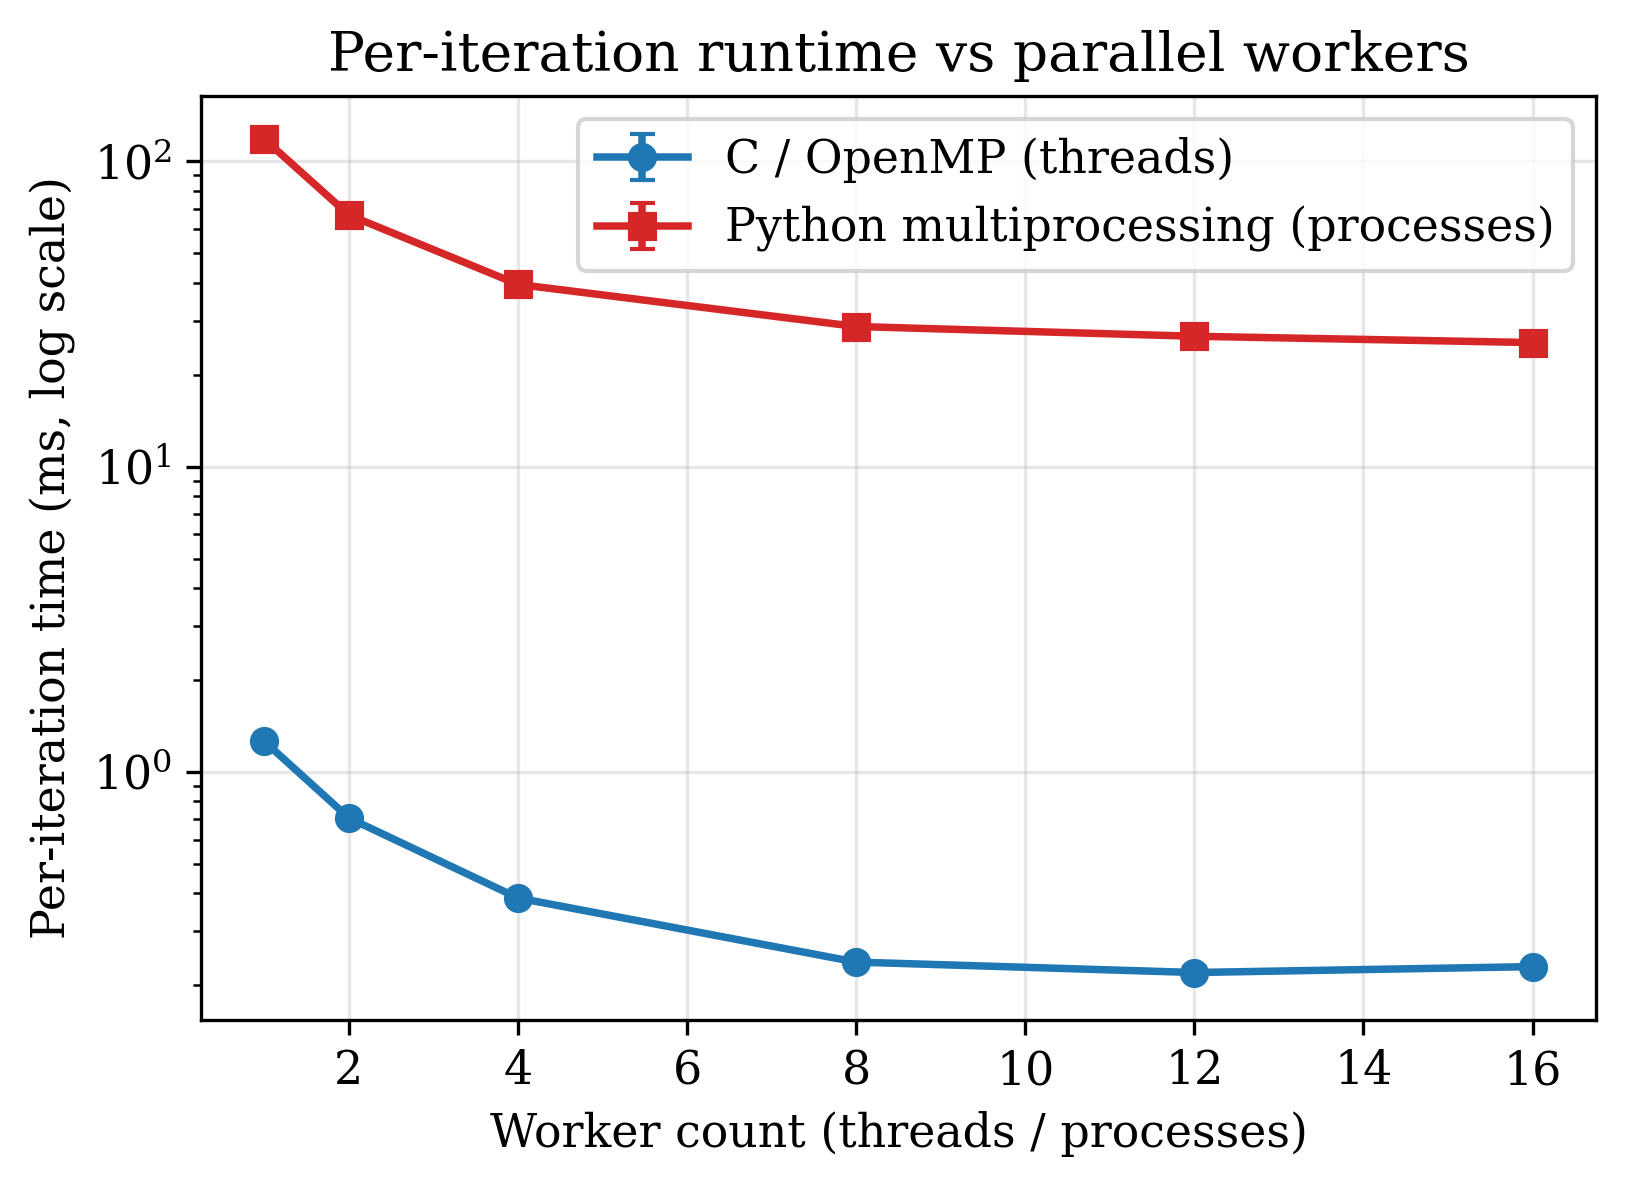
\includegraphics[width=\columnwidth]{fig_runtime.png}
\caption{Per-iteration runtime vs worker count (log scale). C/OpenMP is roughly
two orders of magnitude faster per iteration than Python multiprocessing.}
\label{fig:runtime}\end{figure}

\begin{figure}[t]\centering
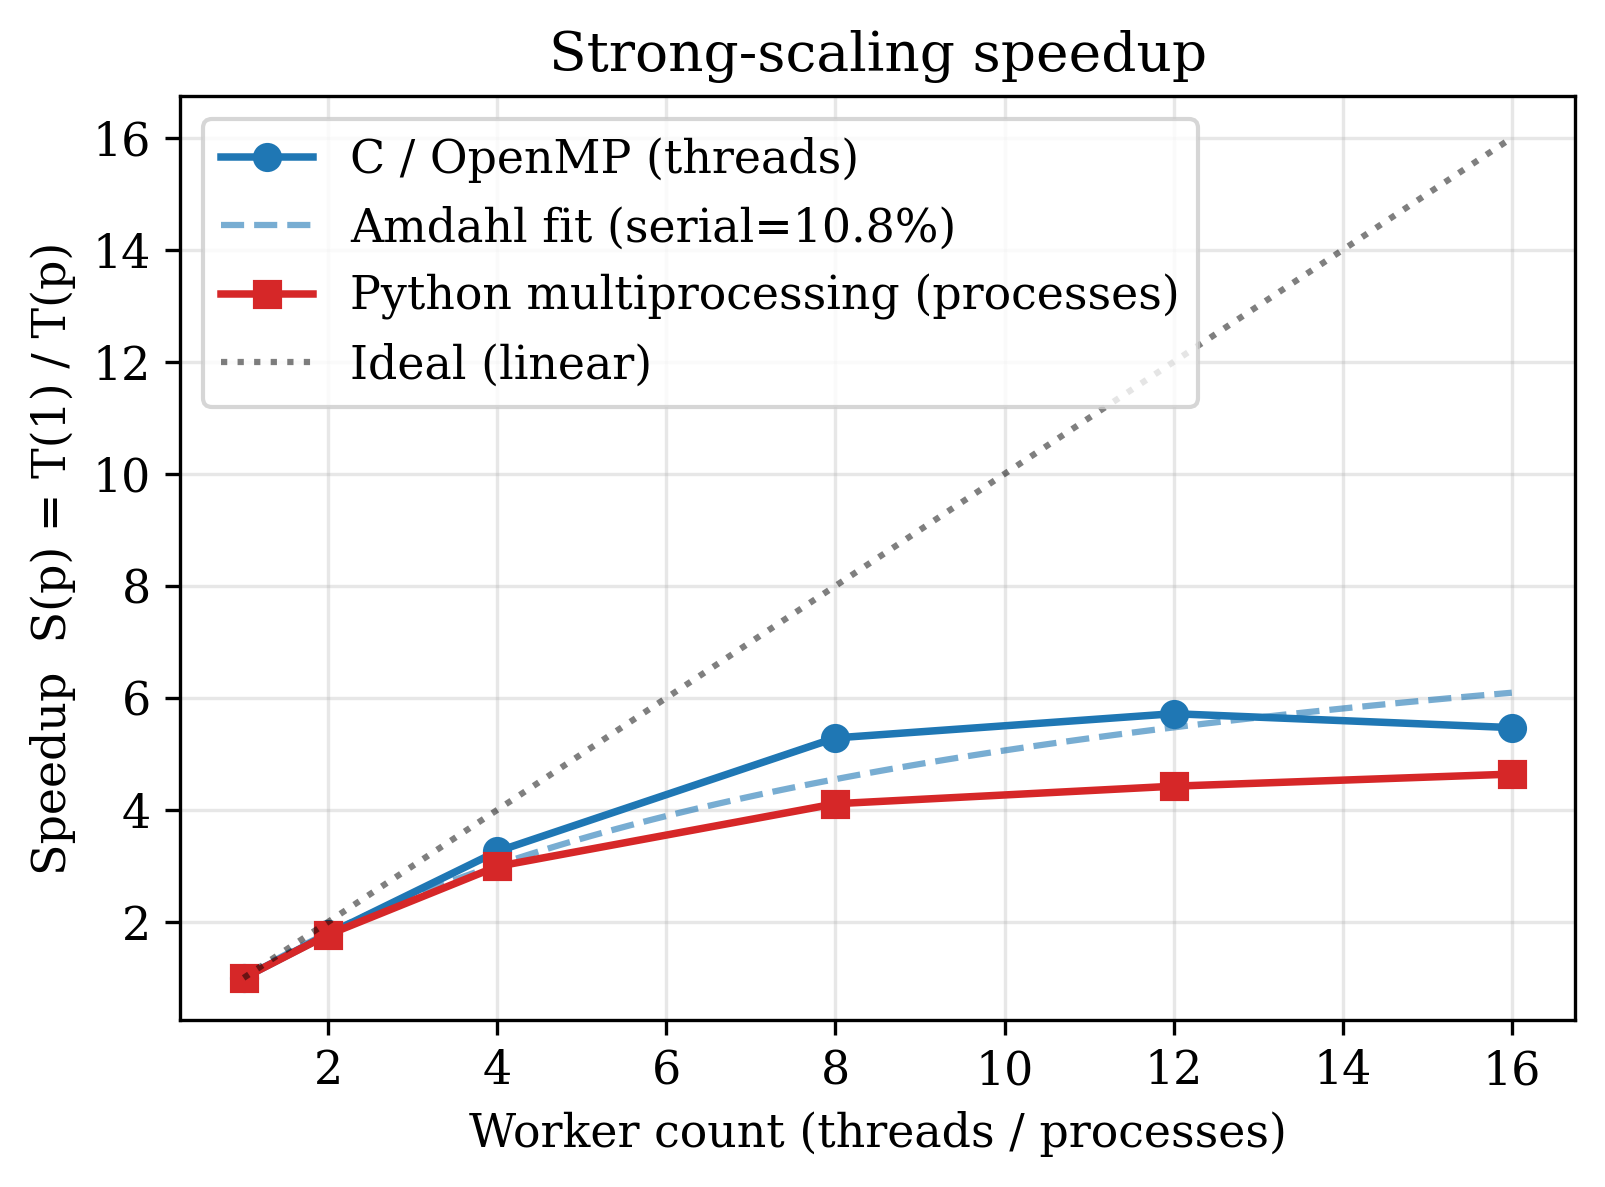
\includegraphics[width=\columnwidth]{fig_speedup.png}
\caption{Strong-scaling speedup with Amdahl's-law fit for C/OpenMP and the ideal
linear reference.}
\label{fig:speedup}\end{figure}

\begin{figure}[t]\centering
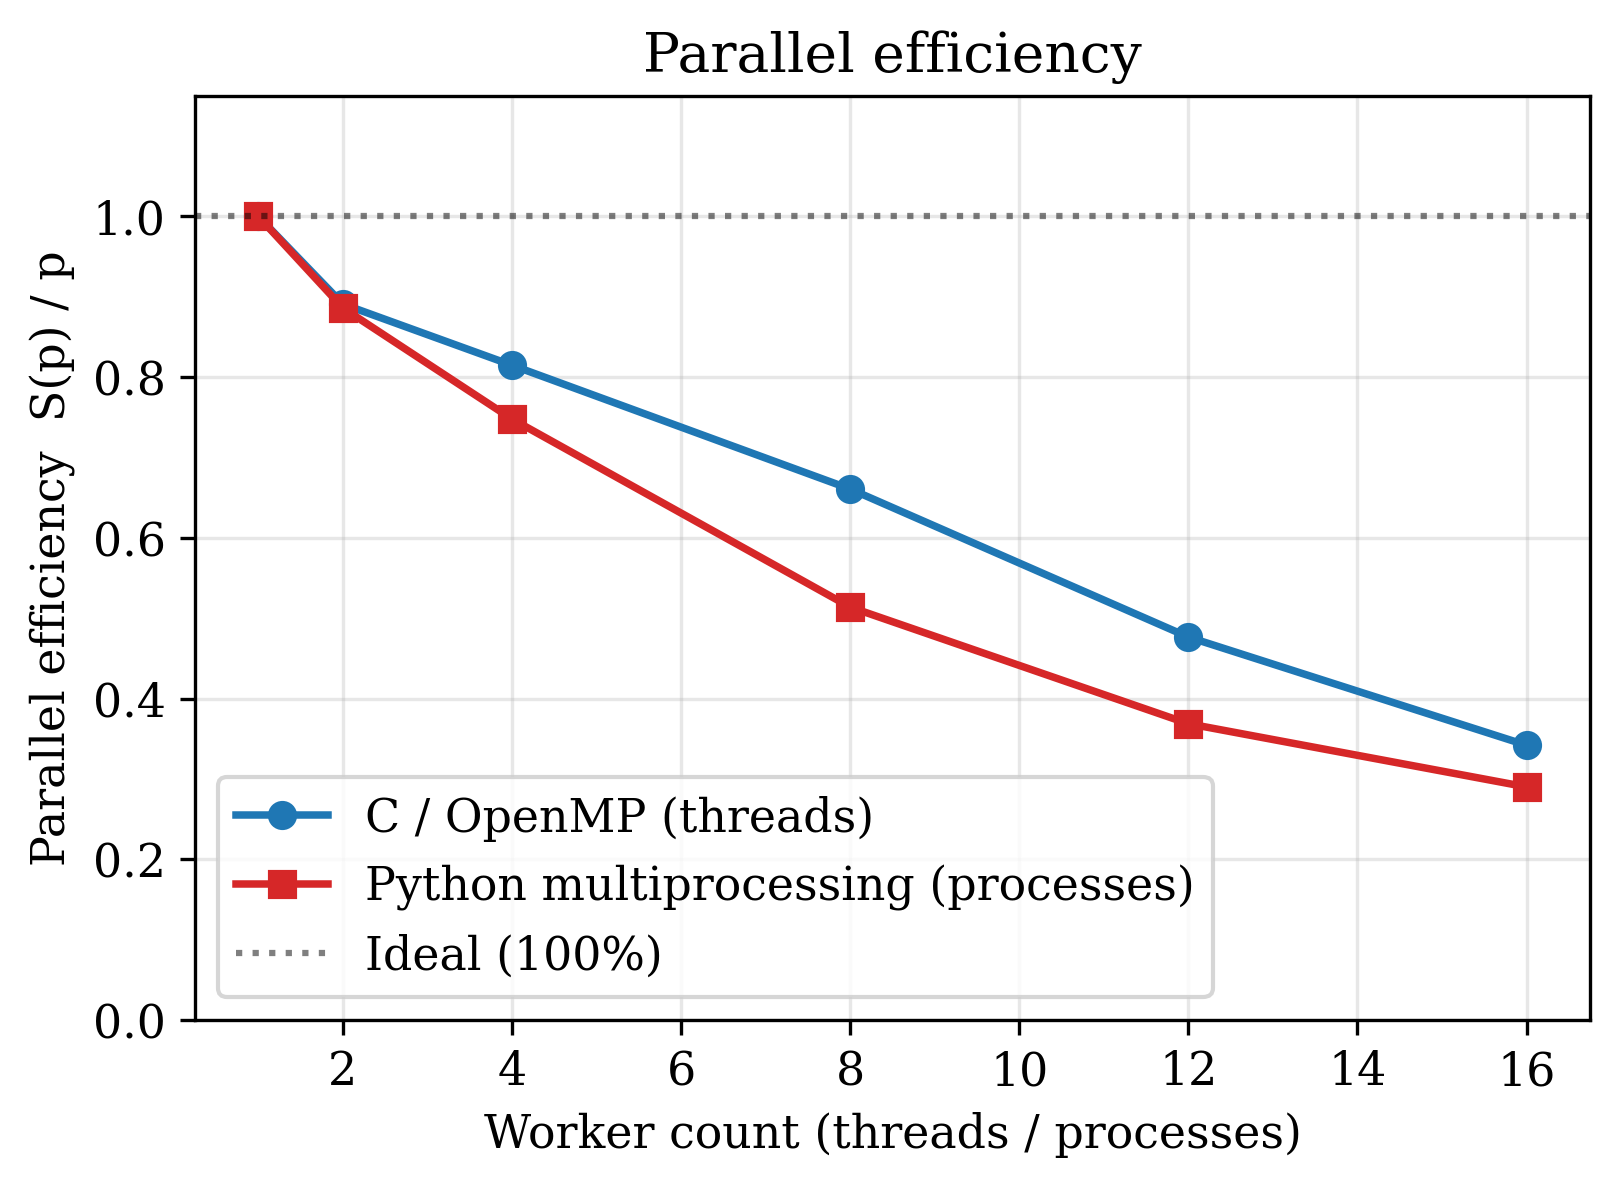
\includegraphics[width=\columnwidth]{fig_efficiency.png}
\caption{Parallel efficiency $S(p)/p$.}
\label{fig:efficiency}\end{figure}

\subsection{Serialization overhead}
Notably, Python \texttt{multiprocessing} with a single worker is \emph{slower}
than the pure-serial Python baseline, because inter-process data transfer is
incurred without any parallel benefit. [[FILL: quote the two numbers.]] This
isolates the cost of process-based parallelism for fine-grained tasks.

\subsection{Solution quality vs obstacle density}
Fig.~\ref{fig:quality} reports best path length as obstacle density increases.
[[FILL: describe the trend and any failure threshold.]]

\begin{figure}[t]\centering
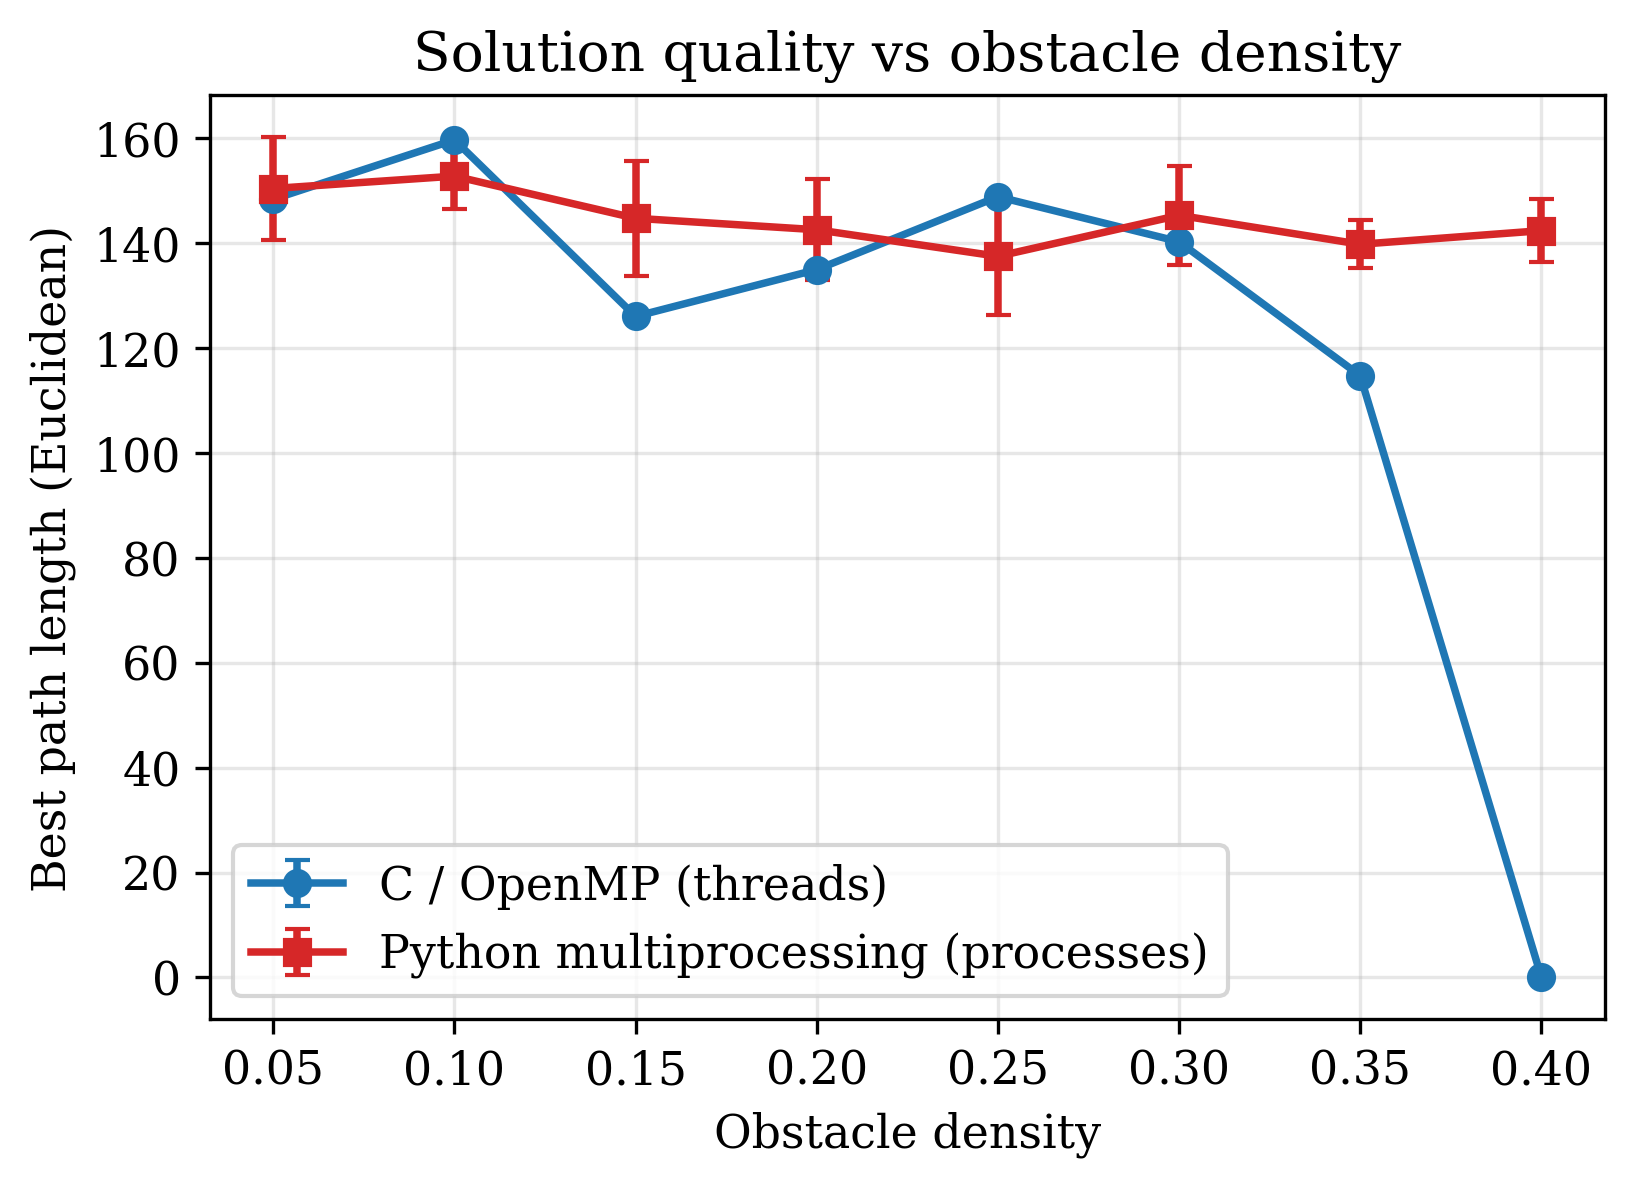
\includegraphics[width=\columnwidth]{fig_quality_density.png}
\caption{Best path length vs obstacle density (mean $\pm$ 95\% CI).}
\label{fig:quality}\end{figure}

% ===========================================================================
\section{Discussion and Limitations}
[[FILL]] The C solver caps the grid at $N\le 50$ (static allocation); larger maps
would require dynamic allocation. The two back-ends generate obstacle layouts
independently, so quality is compared in aggregate rather than per-instance.
Results are single-machine; multi-node/distributed-memory scaling and a GPU
implementation are left to future work.

% ===========================================================================
\section{Conclusion}
We presented a reproducible, controlled comparison of process- and thread-based
parallel ACO for grid path planning. [[FILL: one-paragraph takeaway with the
headline numbers.]]

\bibliographystyle{IEEEtran}
\bibliography{refs}

\end{document}
